\documentclass[mathserif]{beamer}
\usepackage[utf8]{inputenc}
\usepackage{blindtext}
\usepackage{color}
\usepackage{multicol}

\usepackage{listings}
\usepackage{fancyvrb}
\usepackage{graphicx}
\usepackage{xcolor,color}
\definecolor{dkgreen}{rgb}{0,0.6,0}
\definecolor{dkpurple}{rgb}{0.4,0.1,0.4}
\definecolor{blue}{rgb}{0.0,0.0,1.0}

\lstset
{
  tabsize=2,
  basicstyle=\small\ttfamily,
  keywordstyle=\bfseries\color{dkpurple},
  stringstyle=\color{blue},
  commentstyle=\color{dkgreen},
  showstringspaces=false,
}

\setbeamertemplate{note page}[default]
% \setbeameroption{show notes}
% \setbeameroption{show notes on second screen}

% acceptable: default, Hannover, Goettingen, Szeged, Singapore, Boadilla
\usetheme{Hannover}

% acceptable: default, dove, maybe beaver
\usecolortheme{default}

\title{We are Turing Machines}
\author[TC CK]{Tyler~I.~Cecil\\Christopher~Koch}
\institute[New Mexico Tech]{
  Department of Computer Science and Engineering\\
  New Mexico Tech
}
\date{November 10, 2014}
\subject{Computer Science}

\begin{document}
\frame{\titlepage}

\section{Decisions}
\begin{frame}
  \frametitle{What Does it Take to Be a Computer?}

  For people who use computers every day, we need to ask two important questions\ldots

  \begin{enumerate}
    \item But what does it take to \emph{be} a computer?

    \item Are there limits to what computers can do?
  \end{enumerate}
\end{frame}

\begin{frame}
  \frametitle{Kurt G\"odel}

  Questions like this first started being asked when this guy broke modern
  mathematics.

  \vspace{2ex}
  \centerline{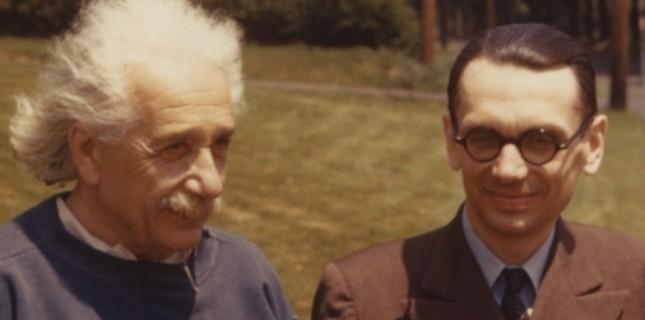
\includegraphics[width=0.8\linewidth]{media/godel.jpg}}
\end{frame}

\begin{frame}
  \frametitle{Entscheidungsproblem}

  \begin{multicols}{2}
    After math broke, Hilbert asked an important question:

    \begin{quote}
      What is the algorithm to decide whether or not a given statement is always
      true?
    \end{quote}

    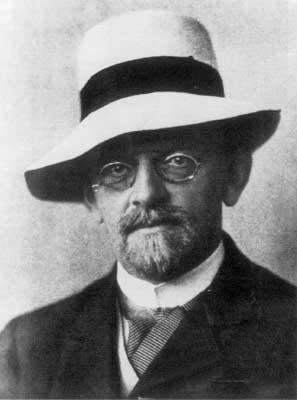
\includegraphics[width=\linewidth]{media/hilbert.jpg}
  \end{multicols}
\end{frame}

\begin{frame}
  \frametitle{Algorithm}
  To do this, we need a formal definition of an algorithm. Thus let
  us define what it means to be ``effectively computable''.

  Many definitions of effective computability were proposed, each stronger than
  the last.
\end{frame}

\section{PDA}
\begin{frame}
  \frametitle{Push-Down Automata}

  Hear is one definition that is often used:

  You get a machine with
  \begin{itemize}
    \item a stack, for memory,
    \item a finite number of states, to represent ``stages'' in the algorithm,
      and
    \item read-only input.
  \end{itemize}
\end{frame}

\begin{frame}
  \frametitle{Push-Down Automata Example}
  Let's try our own!

  \begin{quote}
    \textbf{Task:} Decide if a string of binary is of the form 
      \[ 0^n1^n \]

    \hrule

    \vspace{5mm}

    For example, $000111$ and $0011$ should pass, but $00111$ or $1010$ should
    fail.
  \end{quote}
\end{frame}

\begin{frame}
  \frametitle{Push-Down Automata Example}
  Now a much harder example\ldots

  \begin{quote}
    \textbf{Task:} Decide if a string of binary is of the form
    \[0^n1^n0^n\]
    
    \hrule

    \vspace{5mm}


    For example, $000111000$ and $001100$ should pass, but $000111$ or $0100$
    should fail.
  \end{quote}
\end{frame}

\begin{frame}
  \frametitle{Sorry}

  \centerline{So\ldots that last question was actually impossible!}
\end{frame}

% Give 5 minutes for them to try to figure out a^n b^n c^n

\section{Turing}
\begin{frame}
  \frametitle{Turing and Church}

  After some time of looking for an answer, these two men independently found
  the most powerful kind of algorithms.
  \begin{multicols}{2}
    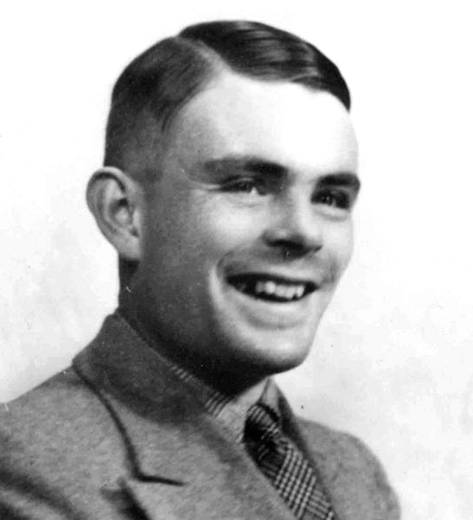
\includegraphics[width=0.9\linewidth]{media/turing.jpg}

    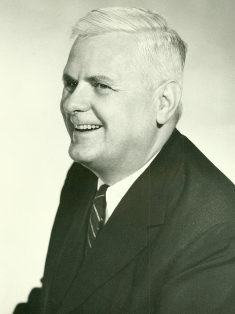
\includegraphics[width=0.9\linewidth]{media/church.jpg}
  \end{multicols}
\end{frame}

\section{Turing Machines}
\begin{frame}
  \frametitle{Turing Machines}

  \begin{itemize}
    \item Alan Turing came up with what is known as \emph{Turing Machines}.

    \item Same thing, but with two stacks!

    \item (Not really, but it's equivalent\ldots)
  \end{itemize}
\end{frame}

\begin{frame}
  \frametitle{Turing Machine Example}

  \begin{quote}
    \textbf{Task:} Add two binary numbers of variable length. 

    Assume the binary numbers are stored in reverse in the read-only input.
  \end{quote}
\end{frame}

\section{Church-Turing}
\begin{frame}
  \frametitle{Church-Turing Thesis}

  \begin{quote}
    Everything that is computable is Turing computable.
  \end{quote}

  Read: There is nothing more powerful than a Turing machine.
\end{frame}

\section{Entscheidungen}
\begin{frame}
  \frametitle{Entscheidungsproblem and Halting}

  Remember the Entscheidungsproblem:
  \begin{quote}
    What is the algorithm to decide whether or not a given statement is always
    true?
  \end{quote}

  Similarly, there is the Halting problem:
  \begin{quote}
    What is the algorithm to decide whether a given arbitrary algorithm will
    halt?
  \end{quote}

  The answer is a bit disappointing:

  {\Large There are no such algorithms.}

\end{frame}

\section{Equivalence}
\begin{frame}
  \frametitle{Equivalence}

  \begin{center}
    (Given Church-Turing thesis, ) To show something is equivalent to a Turing
    machine, you only have to have it simulate a Turing machine.

    \vspace{10mm}

    {\Large You are a Turing Machine!

    But are you more than a Turing machine?}

    {\small Probably not.}
  \end{center}
\end{frame}

\end{document}
